\paragraph{Усовершенствованный алгоритм оценки АКФ}
Точность АР метода напрямую зависит от точности оценки АКФ гармонического сигнала.
Существует несколько способов компенсации шума для АР анализа.
Основным способом повышения точности оценки АКФ является увеличение размера выборки, что в случае модулированного сигнала может быть затруднительным. 

В данной работе предлагается использовать алгоритм увеличения ОСШ методом последовательного вычисления АКФ.
Для снижения вычислительных затрат последовательное вычисление АКФ предлагается реализовывать с использованием процедуры БПФ. 
Введем следующие обозначения: ${x}$ – вектор входного сигнала после снятия ПСП, ${F}$ – матрица прямого преобразования Фурье,
${F^{-1}}$ - матрица обратного преобразования Фурье. Оценку АКФ на первом шаге можно получить следующим образом:

Уточненная оценка АКФ на K-ом шаге данного алгоритма может быть получена с помощью выражения:
\begin{center}
\begin{equation}
	\label{eq:akf_3}
	\hat{r}_K = F^{-1}\left[ \left| Fx \right| ^{2^K} \right]
\end{equation}
\end{center}

Схематически алгоритм получения уточненной оценки АКФ на третьем шаге представлен на рисунке \ref{pic:akf_pic}.
\begin{figure}[H]
	\center\scalebox{0.8}{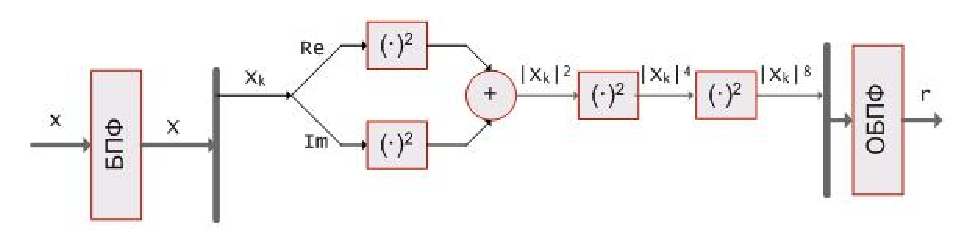
\includegraphics[width=1\linewidth]{akf_fft.eps}}
	\caption{Усовершенствованный итеративный алгоритм получения АКФ}
	\label{pic:akf_pic}
\end{figure}

Количество умножений необходимых для оценки АКФ прямым методом: ${OP_{ACF} = 3N^2}$. Количество умножений необходимых для оценки
усовершенствованным итеративным алгоритмом получения АКФ: ${OP_{ACF\_FFT} = 8NlogN + (k+2)N}$.

Увеличение отношения ОСШ в оценке АКФ по мощности можно вычислить по известной формуле:
\begin{center}
\begin{equation}
	\label{eq:akf_max_eq}
	G=2BT \frac{1}{2+1/SNR_k}
\end{equation}
\end{center}
где ${G=\frac{SNR_{k+1}}{SNR_k}}$ - относительный прирост ОСШ, ${T}$ - длинна выборки (сек), ${B}$ -  ширина спектра сигнала, 
а ${SNR}$ - ОСШ.

Данный алгоритм позволяет вырастить спектральный пик. На рисунке \ref{pic:gps_spectrum} представлен спектр после повторного
модуляции ПСП. В ввиду смещения спектрального пика, оценка параметрическим методом даст смещенное значение. После 3х
итераций предлагаемого алгоритма спектральный пик существенно вырастает над уровнем шума - рисунок \ref{pic:GPS_spectrum_iter3}.

\begin{figure}[H]
	\center\scalebox{0.8}{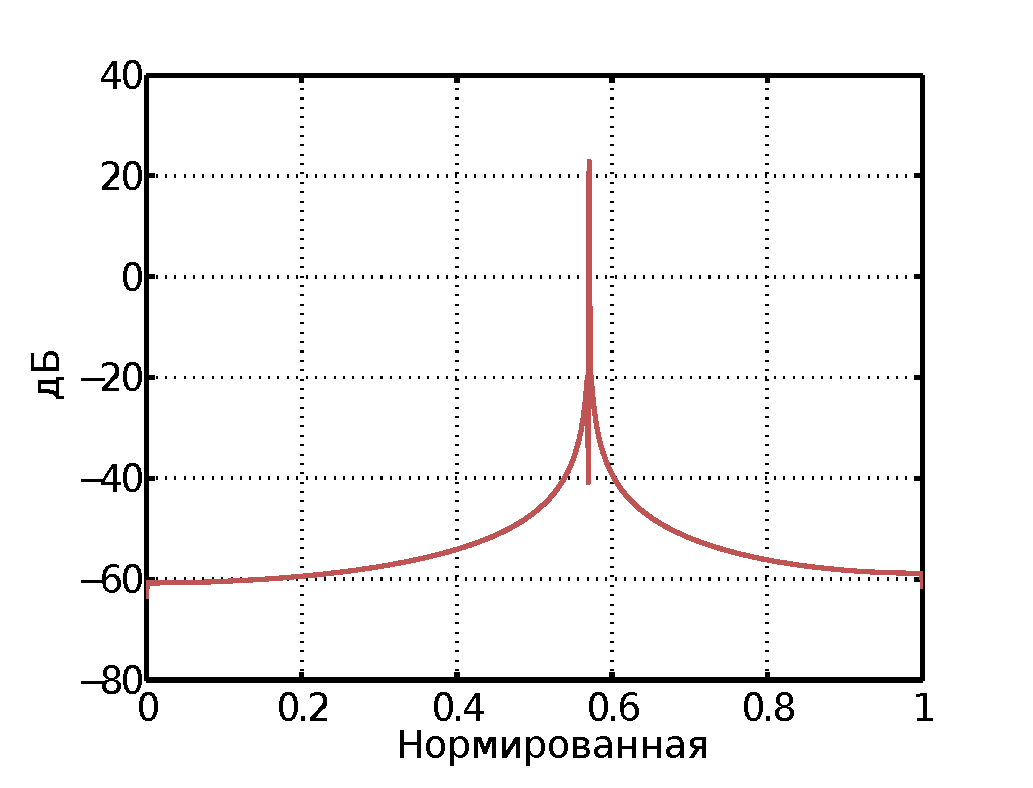
\includegraphics[width=1\linewidth]{GPS_spectra_iter3.eps}}
	\caption{СПМ сигнала после 3 итерации уточнения АКФ}
	\label{pic:GPS_spectrum_iter3}
\end{figure}
